% !BIB TS-program = biber

\RequirePackage[l2tabu,orthodox]{nag}

% TODO: decide if one-sided/two-sided
%\documentclass[headsepline,footsepline,footinclude=false,fontsize=11pt,paper=a4,listof=totoc,bibliography=totoc,BCOR=12mm,DIV=12]{scrbook} % two-sided
\documentclass[headsepline,footsepline=false,footinclude=false,oneside,fontsize=11pt,paper=a4,listof=totoc,bibliography=totoc]{scrbook} % one-sided

% TODO: change citation style in settings
\input{template/settings}

\newacronym{TUM}{TUM}{Technical University of Munich}
\newacronym{CIT}{CIT}{School of Computation, Information and Technology}
\newacronym{ESM}{ESM}{Associate Professorship of Environmental Sensing and Modeling}
\newacronym[longplural=Green House Gases]{GHG}{GHG}{Green House Gas}
\newacronym{LRZ}{LRZ}{Leibniz-Rechenzentrum}
\newacronym{MWN}{MWN}{Munich Scientific Network}

% refer to https://en.wikibooks.org/wiki/LaTeX/Glossary for acronyms and glossary entries
\newglossaryentry{gamma}
{
  name={\ensuremath{\gamma}},
  description={Regularization factor in generative model solver},
  sort=gamma
}

\newglossaryentry{lambda}
{
  name={\ensuremath{\lambda}},
  description={Regularization factor in sparse generative model solver},
  sort=lambda
}



% TODO: change thesis information
\newcommand*{\getUniversity}{Technische Universität München}
\newcommand*{\getChair}{Professorship of Environmental Sensing and Modeling}
\newcommand*{\getDepartment}{Department of Electrical Engineering}
\newcommand*{\getSchool}{Computation, Information and Technology}
\newcommand*{\getTitle}{Thesis title}
\newcommand*{\getTitleGer}{Titel der Abschlussarbeit}
\newcommand*{\getAuthor}{Author}
\newcommand*{\getDoctype}{Bachelor's Thesis, Master's Thesis, \ldots}
\newcommand*{\getAdvisor}{Advisor}
\newcommand*{\getExaminer}{Prof. Dr.-Ing. Jia Chen}
\newcommand*{\getSubmissionDate}{Submission date}
\newcommand*{\getSubmissionLocation}{Munich}

\begin{document}

% Set page numbering to avoid "destination with the same identifier has been already used" warning for cover page.
% (see https://en.wikibooks.org/wiki/LaTeX/Hyperlinks#Problems_with_Links_and_Pages).
\pagenumbering{alph}
\begin{titlepage}
    % HACK for two-sided documents: ignore binding correction for cover page.
    % Adapted from Markus Kohm's KOMA-Script titlepage=firstiscover handling.
    % See http://mirrors.ctan.org/macros/latex/contrib/koma-script/scrkernel-title.dtx,
    % \maketitle macro.
    \oddsidemargin=\evensidemargin\relax
    \textwidth=\dimexpr\paperwidth-2\evensidemargin-2in\relax
    \hsize=\textwidth\relax

    \centering

    \vspace*{5mm}

    \IfFileExists{template/logos/tum-logo-blue.png}{%
        
\includegraphics[height=20mm]{template/logos/tum-logo-blue.png}
    }{%
        \vspace*{20mm}
    }

    \vspace{20mm}

    {\huge\MakeUppercase{TUM School of \getSchool{}} \par}

    \vspace{5mm}
    {\large\MakeUppercase{\getDepartment{}} \par}

    {\large\MakeUppercase{\getChair{}} \par}

    \vspace{15mm}

    {\huge\bfseries \getTitle{} \par}

    \vspace{10mm}
    {\LARGE \getAuthor{}}

\end{titlepage}




\frontmatter{}

\begin{titlepage}
    \centering

    \vspace*{5mm}

    \IfFileExists{template/logos/tum-logo-blue.png}{%
        
\includegraphics[height=20mm]{template/logos/tum-logo-blue.png}
    }{%
        \vspace*{20mm}
    }

    \vspace{20mm}
    {\huge\MakeUppercase{School of \getSchool{}} \par}

    \vspace{5mm}
    {\large\MakeUppercase{\getDepartment{}} \par}

    {\large\MakeUppercase{\getChair{}} \par}

    \vspace{20mm}

    {\huge\bfseries \getTitle{} \par}

    \vspace{10mm}
    {\huge\bfseries \foreignlanguage{ngerman}{\getTitleGer{}} \par}

    \vspace{15mm}

    \begin{tabular}{l l}
        Author:            & \getAuthor{}         \\
        Thesis Supervisor: & \getExaminer{}       \\
        Advisor:           & \getAdvisor{}        \\
        Submission Date:   & \getSubmissionDate{} \\
    \end{tabular}

    \vspace{25mm}
    \IfFileExists{template/logos/esm-logo-square.png}{%
        \vfill{}
        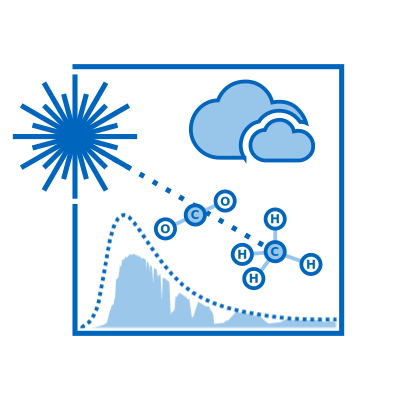
\includegraphics[height=20mm]{template/logos/esm-logo-square.png}
    }{}

\end{titlepage}

\input{template/disclaimer}
\addcontentsline{toc}{chapter}{Acknowledgments}
\thispagestyle{empty}

\vspace*{20mm}

\begin{center}
    {\usekomafont{sectioning}\usekomafont{section} Acknowledgments}
\end{center}

First and foremost, I would like to express my deepest gratitude to my advisor, Moritz Makowski, and professor and supervisor, Prof. Dr. Jia Chen, for their guidance and encouragement.
Their support was incredibly valuable when the challenges at hand seemed almost impossible to overcome.
I am grateful for being entrusted with this novel and challenging idea and for the opportunity to independently research this project.
I do not take this opportunity for granted and am thankful for it.

I also extend my thanks to my friends.
I could not have wished for better ones in my life.
Whenever I faced uncertainties, my friends were my first point of contact.

Lastly, I offer my heartfelt appreciation to my family - my elder brother, my two sisters, and my parents - for their endless love, support, and understanding during tough times.
Although they could not provide much assistance on educational topics throughout my life, I know they would have helped if they could.
They always believed in me, even when I did not believe in myself.
Especially to my parents, I acknowledge how much you have sacrificed to make this education possible and will forever be grateful.
Without my family, this accomplishment would not have been possible.

\vspace{10mm}

\cleardoublepage{}

\chapter{\abstractname}

Dolor aliqua eu labore laboris pariatur velit est est aliquip dolore aliquip minim et. Enim labore adipisicing aliqua anim Lorem. Ex dolor exercitation id cillum consequat laboris. Occaecat id id aute minim sit qui dolore irure pariatur. Enim mollit reprehenderit veniam sunt reprehenderit est aute Lorem dolor veniam.

Laboris ad aliqua fugiat mollit sunt veniam esse cillum excepteur esse do ea veniam. Est ut aliqua culpa ad culpa. Cupidatat ullamco dolore pariatur proident esse minim voluptate dolor ad aliqua incididunt incididunt consequat do. In dolor incididunt in dolore laborum nulla eu nulla dolor fugiat dolore eu.

\clearpage

\glsnogroupskiptrue
\printnoidxglossaries

\clearpage

\microtypesetup{protrusion=false}
\tableofcontents{}
\microtypesetup{protrusion=true}

\mainmatter{}

% !TeX root = ../main.tex
% Add the above to each chapter to make compiling the PDF easier in some editors.

\chapter{Introduction}\label{chapter:introduction}

Global warming poses a significant challenge to our planet and is primarily caused by anthropogenic \gls{GHG} emissions \parencite{IPCC_AR6}.
As a result, climate mitigation has become increasingly important to address this pressing issue.
Emission inventories play an essential role in this effort.
These are collections of emission data of pollutants or \gls{GHG}s released into the atmosphere over a specified period within a defined geographic area.
They serve as foundational tools for environmental management, play a pivotal role in policy formulation, and are essential for compliance with international agreements on climate change mitigation.
Emission inventories are constructed using various techniques, including the bottom-up and downscaling approaches.

The bottom-up approach collects detailed activity data for each emission source, such as fuel consumption rates or industrial production volumes.
Emission factors, representing the average emissions per unit of activity, are then multiplied by these data, resulting in an estimate of the total emissions from that source.
This method enables sectoral analysis, allowing for the identification of crucial emission contributors.

Methods relying on downscaling through spatial proxies, such as those used by the Netherlands Organisation for Applied Scientific Research (TNO) \parencite{TNO_HighRes15, TNO_HighRes18}, start from national-level emission data and disaggregate it to finer spatial scales.
Spatial proxies, such as population density, land use patterns, or road networks, are used to allocate emissions geographically \parencite{SpatialProxies}.

While emission inventories offer detailed estimates, they can be inaccurate due to incomplete data, outdated emission factors, the exclusion of unknown or hidden emission sources, and inaccurate spatial proxy maps \parencite{InventoryUncertainties}.
These limitations underscore the need for inversion techniques, also called top-down approaches.
Top-down approaches promise to close the gap between the actual emissions and those captured by the emission inventories, thus enhancing their comprehensiveness.

Top-down approaches using atmospheric concentration measurements are based on solving ill-posed inverse problems, a widely studied research field.
These approaches formulate the emission estimation problem as an inverse problem, where \gls{GHG} concentrations measured at ground-based or satellite stations are used to infer the underlying emission flux fields based on atmospheric transport.
Examples of sensor networks that perform such measurements include MUCCnet \parencite{MUCCnet} and BEACO\textsubscript{2}N \parencite{BEACON2N}, among others.

From these measurements, top-down approaches reconstruct the emission field by applying inversion techniques.
One such technique is Bayesian inversion, which updates prior knowledge about emissions using a likelihood function derived from measurement data.
Prior knowledge refers to information about emissions before incorporating new measurement data.
However, these methods rely heavily on priors and accurate knowledge about their uncertainties, i.e., assumptions about the emission fluxes, which can introduce bias when information is incomplete or incorrect.

There are many approaches that overcome this limitation of introduced bias, such as geostatistical approaches \parencite{Geostatical}, with recent studies exploring sparse reconstruction techniques \parencite{UrbanSparseReconstruction}. % could add some more here (see Zanger paper)
Sparse reconstruction methods assume that emissions are spatially sparse (i.e., only a few significant sources contribute significantly to the total emissions) and use optimization techniques to recover the emission field from a limited set of measurements.
\textcite{UrbanSparseReconstruction} demonstrated that compressed sensing approaches can be practical for reconstructing \gls{GHG} emissions in urban environments, especially when combined with domain transformations, such as \gls{DWT} \parencite{Wavelets} or \gls{DCT} \parencite{DCT}.

Ill-posed inverse problems arise in many other research fields, including medical imaging.
Significant advancements have been made in this field through machine learning-based compressed sensing techniques \parencite{ReviewCSUsingAI}.
This thesis takes inspiration from these developments and, with advancements in machine learning-based compressed sensing, investigates the applicability of one such approach based on generative models in urban \gls{GHG} emission flux estimation.
The code developed for this research, as well as the model weights, are publicly available on GitHub\footnote{\href{https://github.com/tum-esm/inventory-embeddings}{github.com/tum-esm/inventory-embeddings}}.

% !TeX root = ../main.tex
% Add the above to each chapter to make compiling the PDF easier in some editors.

\chapter{State-of-the-Art}\label{chapter:state-of-the-art}

\section{Section}
Citation test~\parencite{latex}.

Lorem ipsum dolor sit amet, consectetur adipiscing elit. Fusce a porta neque, non eleifend dui. Proin maximus tempus eros, ut vehicula lectus tempor at. Nulla vel sodales neque, ut hendrerit odio. Etiam posuere luctus lectus, ut vestibulum lacus congue in. Donec aliquet lorem at mi efficitur, in lacinia erat congue. Fusce vel quam turpis. Quisque sed leo a erat porttitor tempus eu eu eros. Donec pulvinar auctor porta. Vestibulum ante ipsum primis in faucibus orci luctus et ultrices posuere cubilia curae;
Quisque metus justo, pharetra quis lectus a, tristique convallis diam. Nulla vitae augue faucibus, aliquet urna eu, hendrerit eros. Sed neque nulla, pellentesque pretium finibus quis, efficitur cursus nunc. Duis ac eros at libero porta convallis sed non massa. Pellentesque vitae tristique nulla, quis hendrerit felis. Sed vestibulum, ante et congue pharetra, purus arcu iaculis leo, quis gravida libero orci id nulla. Sed sit amet euismod neque. Praesent rutrum sagittis finibus. Nam ac laoreet turpis. Duis sagittis metus ac gravida ultricies. Donec at sollicitudin risus. Morbi vel metus vel tortor pretium ullamcorper. In hac habitasse platea dictumst. Phasellus feugiat risus id rutrum aliquet. Donec congue urna at urna congue fringilla. Nullam metus ex, scelerisque vel metus non, dignissim aliquam velit.
Pellentesque vulputate est in massa aliquet, eu dignissim purus tempus. Aenean maximus risus sit amet neque pretium, id molestie sapien auctor. Class aptent taciti sociosqu ad litora torquent per conubia nostra, per inceptos himenaeos. Nulla placerat neque vitae fermentum luctus. Duis tincidunt lectus vel neque mattis, et tempus lacus tristique. Morbi accumsan vulputate leo, at cursus libero convallis ut. Nunc quam nulla, commodo a lorem at, eleifend iaculis augue. Quisque non volutpat lectus, ut sodales risus. Ut scelerisque lacinia risus vel fermentum.
Aenean iaculis justo interdum, venenatis erat sit amet, lacinia nulla. Mauris et felis a lorem sodales tempus ut a massa. Mauris tempor urna vel convallis aliquam. Ut aliquam suscipit massa, ac tempus dolor. Sed ornare imperdiet aliquam. Donec ut semper odio. Mauris in elit metus. Donec id justo in nibh feugiat maximus in sollicitudin tortor.
Nunc pellentesque, felis a iaculis molestie, nunc augue ultrices ligula, ac aliquet arcu elit eu libero. Orci varius natoque penatibus et magnis dis parturient montes, nascetur ridiculus mus. Morbi neque odio, bibendum quis maximus nec, condimentum et ipsum. Integer dictum elit quis aliquet molestie. Vestibulum tristique eros vel dictum porttitor. Nullam at ligula ac leo auctor tempus. Quisque venenatis, mi bibendum tincidunt gravida, urna ligula efficitur libero, ac luctus leo arcu sed libero. Nulla vitae odio sollicitudin metus porta aliquam in et tortor. Nam libero odio, ultrices ut diam ut, venenatis tristique ex.
Lorem ipsum dolor sit amet, consectetur adipiscing elit. Fusce a porta neque, non eleifend dui. Proin maximus tempus eros, ut vehicula lectus tempor at. Nulla vel sodales neque, ut hendrerit odio. Etiam posuere luctus lectus, ut vestibulum lacus congue in. Donec aliquet lorem at mi efficitur, in lacinia erat congue. Fusce vel quam turpis. Quisque sed leo a erat porttitor tempus eu eu eros. Donec pulvinar auctor porta. Vestibulum ante ipsum primis in faucibus orci luctus et ultrices posuere cubilia curae;
Quisque metus justo, pharetra quis lectus a, tristique convallis diam. Nulla vitae augue faucibus, aliquet urna eu, hendrerit eros. Sed neque nulla, pellentesque pretium finibus quis, efficitur cursus nunc. Duis ac eros at libero porta convallis sed non massa. Pellentesque vitae tristique nulla, quis hendrerit felis. Sed vestibulum, ante et congue pharetra, purus arcu iaculis leo, quis gravida libero orci id nulla. Sed sit amet euismod neque. Praesent rutrum sagittis finibus. Nam ac laoreet turpis. Duis sagittis metus ac gravida ultricies. Donec at sollicitudin risus. Morbi vel metus vel tortor pretium ullamcorper. In hac habitasse platea dictumst. Phasellus feugiat risus id rutrum aliquet. Donec congue urna at urna congue fringilla. Nullam metus ex, scelerisque vel metus non, dignissim aliquam velit.
Pellentesque vulputate est in massa aliquet, eu dignissim purus tempus. Aenean maximus risus sit amet neque pretium, id molestie sapien auctor. Class aptent taciti sociosqu ad litora torquent per conubia nostra, per inceptos himenaeos. Nulla placerat neque vitae fermentum luctus. Duis tincidunt lectus vel neque mattis, et tempus lacus tristique. Morbi accumsan vulputate leo, at cursus libero convallis ut. Nunc quam nulla, commodo a lorem at, eleifend iaculis augue. Quisque non volutpat lectus, ut sodales risus. Ut scelerisque lacinia risus vel fermentum.
Aenean iaculis justo interdum, venenatis erat sit amet, lacinia nulla. Mauris et felis a lorem sodales tempus ut a massa. Mauris tempor urna vel convallis aliquam. Ut aliquam suscipit massa, ac tempus dolor. Sed ornare imperdiet aliquam. Donec ut semper odio. Mauris in elit metus. Donec id justo in nibh feugiat maximus in sollicitudin tortor.
Nunc pellentesque, felis a iaculis molestie, nunc augue ultrices ligula, ac aliquet arcu elit eu libero. Orci varius natoque penatibus et magnis dis parturient montes, nascetur ridiculus mus. Morbi neque odio, bibendum quis maximus nec, condimentum et ipsum. Integer dictum elit quis aliquet molestie. Vestibulum tristique eros vel dictum porttitor. Nullam at ligula ac leo auctor tempus. Quisque venenatis, mi bibendum tincidunt gravida, urna ligula efficitur libero, ac luctus leo arcu sed libero. Nulla vitae odio sollicitudin metus porta aliquam in et tortor. Nam libero odio, ultrices ut diam ut, venenatis tristique ex.
% !TeX root = ../main.tex
% Add the above to each chapter to make compiling the PDF easier in some editors.

\chapter{Methods}\label{chapter:methods}

\section{Section}
Citation test~\parencite{latex}.


\input{chapters/04_results}
\input{chapters/05_discussion}
% TODO: add more chapters here

\appendix{}

\microtypesetup{protrusion=false}

%\addchap{Abbreviations}
%\begin{acronym}
%\itemsep-.25\baselineskip
%\acro{TUM}[TUM]{Technical University of Munich}
% TODO: add acronyms
%\end{acronym}

\listoffigures{}
\listoftables{}
\microtypesetup{protrusion=true}
\printbibliography{}

\end{document}
